\chapter*{Introduction}
\addcontentsline{toc}{chapter}{Introduction}
\fancyhead[RE]{\textbf{Introduction}}
\fancyhead[LO]{} 

\section*{2D architecture, current design flows and their limitations}
In order to continuously improve the performance of integrated circuits (IC), technologists deploy enormous efforts to produce IC manufacturing process that is compelling to follow the well-known Moore's Law (see Figure \ref{fig:mooreslaw}). This empirical law predicts a doubling of the transistors' integration each 18 months and therefore increasing logic capacity of the circuit per unit area. 

\begin{figure}
\begin{center}
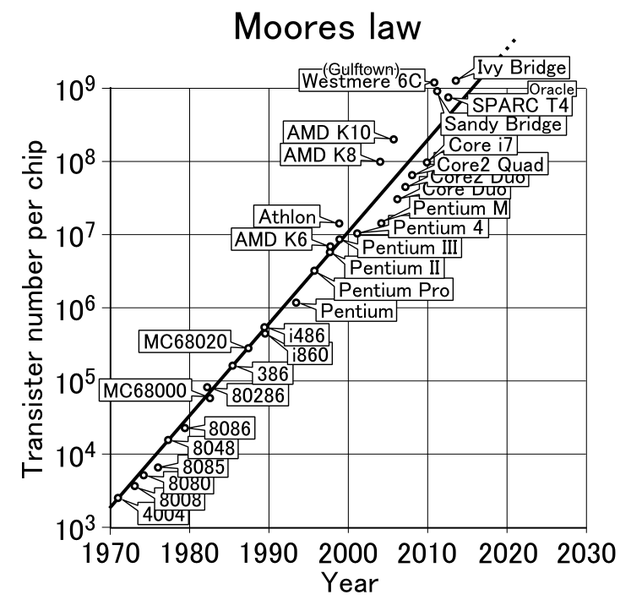
\includegraphics[width=0.75\linewidth]{mooreslaw.png}
\end{center}
\vspace{-0.5cm}
\caption{Moore's law \cite{mooreslawpic}}
\label{fig:mooreslaw}
\end{figure}

The improvements of 2D architectures are primarily driven by the reduction of the transistor size. By reducing transistor dimensions, the switching speed is increased thanks to the shorter distance between the source and the drain, implying an improvement of the overall speed of the designs.

However, as the transistor size is decreasing, the observed improvement is also getting smaller. Indeed, a smaller transistor allows higher device density but will slightly decrease the dynamic and increase the total delay (sum of gate and interconnection delays) at the level of the complete circuit. Also, power consumption is increased due to higher leakage and increasing interconnection wire length \cite{5227192}. In Figure \ref{fig:delaygateinterconnect} is shown the trends in transistor gate delay and interconnect delay with IC fabrication technology where the crossover point represents the interconnect bottleneck \cite{kirchain2007}.

\begin{figure}
\begin{center}
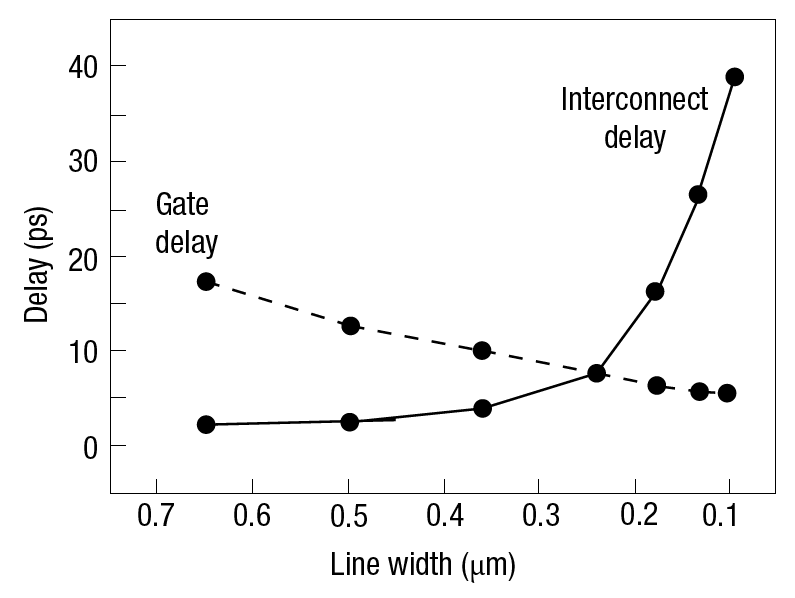
\includegraphics[width=0.75\linewidth]{delaygateinterconnect}
\end{center}
\caption{Trends in transistor gate delay and interconnect delay with IC fabrication technology \cite{kirchain2007}}
\label{fig:delaygateinterconnect}
\end{figure}

With the miniaturization, quantum effects such as quantum tunnelling will significantly affect how a transistor behave \cite{1240081}.

In addition to these physical aspects, economical considerations that will hinder the IC evolution beyond 20nm have to be taken into account \cite{5227192,PFF10}.

In order to overcome these limitations, new technologies have been proposed such as the carbon nanotubes \cite{tans1998room}, the nanowire transistors \cite{doi:10.1021/nl025875l}, the single-electron transistors \cite{citeulike:4194929}, but also the 3D-Stacked Integrated Circuits (3D-SIC) proposed by the academic and industrial communities. The latter has been often cited as the most prominent one~\cite{659500}.

Fast evolution of IC manufacturing technologies makes even the design of 2D-ICs a complex and tedious task with the growing number of design choices at the system level (e.g. number and type of functional units and memories, type and topology of the interconnection system, etc.) and physical level (respecting area/timing/power constraints). Using 3D-SICs introduces even more degrees of freedom: number of tiers, choices for manufacturing technology (e.g. full 3D integration, silicon interposer, face-to-face, back-to-face, etc.), 3D partitioning and placement strategies etc. These new degrees of freedom will contribute to the combinatorial explosion of already huge design spaces. Moreover, practice and 2D design experience cannot be fully exploited with 3D technology, since 3D-SICs change considerably the way ICs are implemented. The current design flows, which already showed their limits with conventional 2D-ICs, may thus need improvements to be able to deal with the increased complexity of emerging 3D-SICs \cite{vanderbiest06, PFF10}.

One of the solutions to face this problem is to develop high-level tools which can quickly explore design spaces and give early and reasonably accurate performance estimations based on physical prototyping of the 3D circuits~\cite{PFF10}.

In addition, performance estimation/optimization and the selection of the most-suitable solutions usually implies to take several objectives in account (e.g. maximization of the performance, minimization of the cost, minimization of the package size, etc.).

Currently, the design tools can be considered to follow a uni-criterion paradigm. Indeed, they have sequential development steps and each criterion is optimized without considering the impact on other criteria. This can lead to several rollbacks in the design flow since the achievement of the requirements can be time consuming (typical design iterations are measured in weeks).

On the other hand, multi-criteria approaches have been developed to optimize all the criteria simultaneously. Designing 3D-SICs inherently implies a huge design space and numerous degrees of freedom and criteria. This is the reason why we propose to apply this paradigm for the design of 3D-SICs.

\section*{Research questions}
Multi-objective optimization and multi-criteria decision aid were developed from the need of taking into account several criteria simultaneously. These tools from the operations research field have shown their abilities in solving similar problems in other fields, which also have a large solution space and applying metaheuristics have shown interesting results~\cite{talbi09}.

In this thesis, we will show the applicability of a multi-criteria paradigm for the design of 3D-SICs:
\begin{itemize}
\item how a 3D circuit can be modelled to apply multi-objective optimization
\item what kind of information can be provided to a designer
\item how multi-criteria decision aid can exploit these results to assist a designer
\end{itemize}

\section*{Outline}
In the first chapter, we will take an overview of the design and manufacturing of 3D-SICs. We will explain the limitations of current design flows and present the developments that have been carried out to overcome these problems. We will discuss why they should be improved and introduce how a multi-criteria paradigm can be useful.

In the chapter two, we will present an overview of the main tools in the MCDA fields where some of the most-used methods will be presented.

In the third chapter, we will define the problem we tackle (the 3D floorplanning) with the considered criteria. We will then show how a 3D-SIC can be modelled in order to apply multi-objective optimization. Simulations will be run on a case study and show what kind of information can be provided to a designer. The methodology will then be validated with a realistic case study to show the added value of a multi-criteria paradigm compared to a uni-criterion approach.

In the chapter four, we will show the robustness of the methodology and the associated algorithms. We will use classical indicators of the fields to analyse the convergence and diversity properties.

In the fifth chapter, we will explain how the obtained results can be exploited using multi-criteria decision aid. We will discuss on how such a paradigm can be used for designing circuits and what needs to be done in order to integrate it to actual design flows.

Finally, we will conclude on the results of the thesis and express some possible perspectives.

